% =====================================================================
%  CSC_43M04_EP — Computer Vision with Deep Learning (École Polytechnique)
%  Team 8 — Florian Guillaumey & Andrea Signoretti
%  Report: two-track report (Closed World + Open World).
%
%  CVPR double-column template.
%
%  Build (from docs/report/):
%    export TEXINPUTS="$PWD:" BSTINPUTS="$PWD:" BIBINPUTS="$PWD:"
%    pdflatex report && bibtex report && pdflatex report && pdflatex report
%
%  Figures live in docs/report/figures/.
% =====================================================================
\documentclass[10pt,twocolumn,letterpaper]{article}

\usepackage{cvpr}
\usepackage{graphicx}
\usepackage{amsmath,amssymb}
\usepackage{booktabs}
\usepackage{xcolor}
\usepackage[pagebackref,breaklinks,colorlinks,allcolors=blue]{hyperref}

\graphicspath{{figures/}}

\def\cvprPaperID{8}
\def\confName{CSC\_43M04\_EP --- Modal d'informatique}
\def\confYear{2026}

\title{What Happens Next? Closed- and Open-World Video Action Recognition\\
on a 33-Class Something-Something\,V2 Subset}

\author{%
Florian Guillaumey\\
\'{E}cole Polytechnique --- Team 8\\
{\tt\small florian.guillaumey@polytechnique.edu}
\and
Andrea Signoretti\\
\'{E}cole Polytechnique --- Team 8\\
{\tt\small andrea.signoretti@polytechnique.edu}
}

\begin{document}
\maketitle
\vspace{-1.2em}
\begin{center}\small May 27, 2026\end{center}

% =====================================================================
\begin{abstract}
We present a two-track study of temporal action prediction on a 33-class subset of
Something-Something\,V2~\cite{goyal2017ssv2}, where only the first ${\approx}40\%$
of each clip (four JPEG frames) is given.
In \textbf{Track~A (Closed World)}, all models are trained from scratch.
We show that two data-centric decisions dominate architecture:
a regularisation warm-up ($+36.3$\,pp) and matching the model's frame count to the
real clip length ($+4.4$\,pp, beating a $2\times$ capacity scale-up).
A five-model log-softmax ensemble combining two TSM architectures (ResNet18 and
ResNet50), one VideoFormer-Lite, and one CE-trained TSM ablation reaches
\textbf{46.75\%} top-1 on the official validation set; the best single model
(TSM-ResNet50, rotating folds) reaches \textbf{42.85\%}.
In \textbf{Track~B (Open World)}, we fine-tune V-JEPA\,2~\cite{bardes2025vjepa2}
and VideoMAE~\cite{tong2022videomae} with progressive unfreezing and
layer-wise learning-rate decay, reaching \textbf{0.6586} Kaggle top-1 with
a 14-model ensemble (16th place in both tracks).
\end{abstract}

% =====================================================================
\section{Problem Description}
\label{sec:problem}

\paragraph{Task.}
The challenge classifies four-frame JPEG clips into 33 motion-defined
action classes (e.g.\ \emph{Pouring something into something}, \emph{Pulling
from left to right}). Each clip contains only the \emph{anticipatory} portion of
the source SSv2 video (shipped \texttt{frame\_003} sits at median frame fraction
$0.40$), so the outcome is deliberately withheld.
The task thus requires reasoning about ongoing motion, not recognising a final
state~\cite{goyal2017ssv2}.

\paragraph{Dataset.}
The split provides $44{,}993$ training, $6{,}745$ validation and $6{,}913$ test
clips over 33 classes. Classes are heavily imbalanced: the largest has $3{,}170$
examples and the smallest only $162$ (ratio $\approx\!20\times$). The KL divergence
between train and validation class distributions is $0.088$, confirming the
splits are representative.

\paragraph{Evaluation and tracks.}
Kaggle scores top-1 accuracy on public+private leaderboard.
\textbf{Track~A (Closed World)} prohibits pretrained models and external data.
\textbf{Track~B (Open World)} permits pretrained backbones and external corpora
but not future frames or test labels.
The task is fundamentally hard for three reasons:
(i) the labels are motion-defined, not appearance-defined;
(ii) four frames is far fewer than the 8--32 used in standard video recognition;
(iii) the decisive cue---the action's outcome---is withheld by design.

% =====================================================================
\section{Methods}
\label{sec:method}

\subsection{Track A --- Closed World}
\label{sec:trackA}

\paragraph{Architecture overview.}
We implemented and compared three temporal architectures, all built on a ResNet
backbone~\cite{he2016resnet} and accepting input clips of shape
$(B, T, C, H, W)$ with $T{=}4$, $H{=}W{=}224$.

\noindent\textbf{CNNBaseline.}
A ResNet18 processes each frame independently, and the $T$ frame-level feature
vectors (each of size $512$) are averaged before the classifier head.
This gives a 0-parameter temporal operation but captures no inter-frame dynamics.
Total: $\approx\!11.2$\,M parameters.

\noindent\textbf{TSM-ResNet (Temporal Shift Module)~\cite{lin2019tsm}.}
The key idea is to inject temporal information \emph{before} each residual block,
while all spatial features are still present at full resolution.
Concretely, for a feature map $\mathbf{x} \in \mathbb{R}^{B \times T \times C
\times H \times W}$, the TSM operation shifts a fraction $1/\text{fold\_div}$ of
channels along the time axis before each convolution:
\begin{equation}
  \text{TSM}(\mathbf{x})_{t,c} = \begin{cases}
  \mathbf{x}_{t-1,c} & c < C/4 \quad \text{(backward shift)} \\
  \mathbf{x}_{t+1,c} & C/4 \leq c < C/2 \quad \text{(forward shift)} \\
  \mathbf{x}_{t,c}   & \text{otherwise}
  \end{cases}
  \label{eq:tsm}
\end{equation}
This adds \textbf{zero parameters and zero FLOPs}: temporal mixing is free.
After 8 residual blocks (each preceded by TSM), a global average pool produces
one 512-d vector per frame; the $T$ vectors are then averaged and a linear head
($512 \!\times\! 33$) produces class logits.

We ran two backbone variants:
\begin{itemize}
  \item \textbf{TSM-ResNet18}: ResNet18 backbone~\cite{he2016resnet},
        $\approx\!11.2$\,M parameters total.
  \item \textbf{TSM-ResNet50}: ResNet50 backbone, $\approx\!23.6$\,M parameters
        (of which $23.5$\,M in the backbone, $0.07$\,M in the head).
        The head is now $2048 \times 33$ due to ResNet50's wider final layer.
\end{itemize}
Both add zero parameters from TSM; the full parameter count comes from the
ResNet backbone and the linear head alone.

\noindent\textbf{VideoFormer-Lite (VFL).}
VFL separates spatial and temporal processing into two explicit stages
(Fig.~\ref{fig:arch}).
\emph{Stage 1 (spatial):} ResNet18 processes each frame independently, producing
$T$ feature vectors of size $d{=}512$ after global average pooling.
\emph{Stage 2 (temporal):} A learnable \texttt{[CLS]} token is appended, giving a
sequence of $T{+}1{=}5$ tokens. A stack of $n_\ell$ pre-norm Transformer
blocks~\cite{xiong2020prenorm} then performs global self-attention over all frames simultaneously.
Each block contains multi-head attention (8 heads) and an MLP
(expansion ratio $r{=}4$), and its parameter count is:
\begin{equation}
  P_{\text{block}} = \underbrace{4d^2}_{\text{Q,K,V,O proj.}} +
  \underbrace{2\,r\,d^2}_{\text{MLP}} + \underbrace{4d}_{\text{layer norms}}
  \approx (4 + 2r)\,d^2
  \label{eq:vfl_params}
\end{equation}
With $d{=}512$, $r{=}4$: $P_{\text{block}} \approx 3.1$\,M. For $n_\ell{=}3$
blocks the Transformer adds ${\approx}9.4$\,M parameters on top of the
${\approx}11.2$\,M ResNet18 backbone, for a total of ${\approx}20.7$\,M.

\paragraph{Where temporal mixing happens --- the key difference.}
TSM mixes time at every spatial resolution, inside every residual block,
\emph{before} any spatial pooling. After 8 blocks of depth, each frame's
representation already encodes a receptive field spanning all $T$ frames.
VFL instead pools all spatial information first, then applies global attention
over the $T{+}1$ pooled vectors. This means VFL sees motion only at the
level of frame-averaged features, while TSM sees it at each $(h, w)$ location.
This distinction matters for SSv2: motion cues like a finger moving or an
object edge displacing live in local spatial regions that are lost after pooling.

\paragraph{Critical frame-count fix ($+4.4$\,pp).}
The clips contain exactly four real frames. Setting \texttt{num\_frames}$\,{>}\,4$
triggers linspace interpolation in the dataset loader, which silently duplicates
frames. For TSM, duplicated frames produce two consecutive tokens with identical
content; the shift in Eq.~\eqref{eq:tsm} then reads the same value twice,
contributing zero temporal gradient for those channel positions.
Fixing \texttt{num\_frames}$\,{=}\,4$ improved internal val by $+4.41$\,pp
($53.32{\rightarrow}57.73\%$) and \texttt{val\_dir} by $+3.34$\,pp.
Scaling to ResNet50 at $T{=}8$ with a fixed split \emph{regressed} to
$45.26\%$ internal (Fig.~\ref{fig:permodel}), confirming that corrupted
temporal input cannot be fixed by larger capacity.
After correcting this, a TSM-ResNet50 at $T{=}4$ with rotating folds reaches
\textbf{42.85\%} \texttt{val\_dir}---the new best single model (Fig.~\ref{fig:backbone}).

\paragraph{Regularisation recipe.}
The most critical element is a \emph{warm-up delay} on MixUp~\cite{zhang2018mixup}
and CutMix~\cite{yun2019cutmix}: both are disabled for the first 10 epochs.
Without it, VFL stalls at $9.45\%$ (killed at epoch 4) vs.\ $45.78\%$ with it
($+36.3$\,pp). The mechanism is straightforward: MixUp creates interpolated labels
(e.g.\ 60\% class A, 40\% class B) that a randomly initialised network cannot
resolve, preventing basic feature formation. The remaining stack (Table~\ref{tab:recipe})
includes focal loss~\cite{lin2017focal} ($\gamma{=}2$, concentrating gradient on
confusable pairs), label smoothing, RandAugment, stochastic depth and AdamW with
cosine warm restarts~\cite{loshchilov2017sgdr}. Horizontal flip is disabled:
it would invert direction-encoded class labels (e.g.\ left$\rightarrow$right
becomes right$\rightarrow$left).

\begin{table}[t]
\centering\small
\setlength{\tabcolsep}{4pt}
\begin{tabular}{@{}lll@{}}
\toprule
Technique & Setting & Source \\
\midrule
Reg.\ warm-up      & 10\,ep, no MixUp/CutMix & \textbf{this work} \\
MixUp / CutMix     & $\alpha{=}0.2$ / $p{=}0.25$, after\,ep\,10 & \cite{zhang2018mixup,yun2019cutmix} \\
Focal loss         & $\gamma{=}2$ & \cite{lin2017focal} \\
Label smoothing    & $\varepsilon{=}0.1$ & \cite{muller2019labelsmooth} \\
RandAugment        & 2 ops, mag.\,0.5 & \cite{cubuk2020randaugment} \\
Stochastic depth   & DropPath 0.1 & \cite{huang2016stochdepth} \\
Optimiser          & AdamW, $\eta{=}10^{-3}$, cosine WR & \cite{loshchilov2019adamw} \\
Horizontal flip    & \textbf{disabled} & label semantics \\
\bottomrule
\end{tabular}
\caption{Track~A training recipe. Reg.\ warm-up is our contribution; all other
components are standard practices from the cited works.}
\label{tab:recipe}
\end{table}

\paragraph{Rotating folds.}
Instead of a fixed 80/20 train/val split, we train with a rotating validation
fold: each epoch the held-out fold shifts by one index (5 folds, so fold$_t =
t \bmod 5$). This ensures every sample participates in $100\%$ of training epochs
rather than $80\%$, with no fixed validation oracle. Model selection uses the
rolling average of the last 5 validation accuracies (one complete rotation).
This adds $+1.2$\,pp for TSM and $+4.3$\,pp for VFL; VFL benefits more
because its global-attention head is data-hungry and lacks the structural
temporal prior that TSM's shift provides.

\paragraph{Track~A ensemble.}
The best five-model ensemble fuses checkpoints by log-softmax late fusion.
Three models use 10-crop TTA (5 spatial crops $\times$ 2 flips):
\texttt{TSM-ResNet18-v2}, its rotating-fold variant, and
\texttt{VFL-Ultra-rotating}. Two run without TTA:
\texttt{TSM-ResNet50-rotating} and a CE-trained TSM ablation model.
Averaging in log-probability space down-weights over-confident wrong predictions
more than raw logit averaging does. The ensemble reaches \textbf{46.75\%} on
\texttt{val\_dir} (Fig.~\ref{fig:ensemble}).

\subsection{Track B --- Open World}
\label{sec:trackB}

We selected two self-supervised families:
\textbf{VideoMAE}~\cite{tong2022videomae} (masked-autoencoder pre-training on
Kinetics-400~\cite{kay2017kinetics}) and
\textbf{V-JEPA\,2}~\cite{bardes2025vjepa2}, which reconstructs masked regions in
\emph{feature} space rather than pixel space, using the self-supervised
\texttt{vjepa2-vitl-fpc64-256} checkpoint without any SSv2 labels
(integrity requirement, Sec.~\ref{sec:integrity}).

\paragraph{Progressive unfreezing with LLRD.}
We fine-tune V-JEPA in three phases with layer-wise LR decay (LLRD), where
block $\ell$ receives $\eta\cdot\lambda^{\ell}$ ($\lambda{=}0.75$).
Phase~0 (frozen backbone, head only): $0.672$ EMA internal val.
Phase~1 (top-6 blocks unfrozen): $0.705$.
Phase~2 (full encoder): $0.728$ internal, $0.6411$ \texttt{val\_dir}.

\paragraph{Window-capped source-frame re-extraction.}
V-JEPA benefits from 16 input frames. We re-extract 16 frames per clip from
the source WebM files, hard-bounded to $[0, \text{window\_end}]$ where
\texttt{window\_end} is located by matching \texttt{frame\_003} against source
frames by pixel-level MAE, and capped at $50\%$ of the source clip so the
withheld outcome is unreachable.

\paragraph{Pseudo-labelling.}
Soft labels from the Phase-2 ensemble are used for test clips with max
confidence $\geq 0.85$; V-JEPA-pseudo reaches $0.6410$ Kaggle.
The growing \texttt{val\_dir}$\rightarrow$Kaggle gap warned against further iterations.

\paragraph{Cross-preprocessing ensemble.}
The final 14 checkpoints come from three families with distinct preprocessing
chains (V-JEPA: 16-frame 256\,px; VideoMAE: 4-frame 224\,px; TSM-ResNet50:
4-frame). Uniform averaging of softmax tensors reaches $0.6586$.

\subsection{Reused vs.\ own code}
We \emph{reuse}: the course starter repository (Hydra configuration,
\texttt{VideoFrameDataset}, \texttt{train.py} skeleton); torchvision ResNet
and R(2+1)D backbones; HuggingFace V-JEPA\,2 and VideoMAE checkpoints (Track~B).
Our \emph{own contributions}: the TSM block wrapper (reimplemented from Lin~et~al.~\cite{lin2019tsm});
VideoFormer-Lite; the regularisation warm-up recipe; rotating $k$-fold training;
log-softmax ensemble and 10-crop TTA pipeline; and the full Track~B stack
(window-capped re-extraction, LLRD fine-tuning, pseudo-labelling loop).

% =====================================================================
\section{Results}
\label{sec:results}

\paragraph{Overall.}
Table~\ref{tab:summary} reports headline results. Track~A reaches
\textbf{46.75\%} on \texttt{val\_dir} from scratch; Track~B reaches
\textbf{0.6586} Kaggle top-1 with the 14-model uniform ensemble.
The gap between tracks (${\approx}20$\,pp) quantifies the practical value of
large-scale pretraining unavailable in the closed track.

\begin{table}[t]
\centering\small
\setlength{\tabcolsep}{5pt}
\begin{tabular}{@{}clcc@{}}
\toprule
Trk & Method & val\,dir & Kaggle \\
\midrule
A & TSM-R18, single best      & 41.68\%  & --- \\
A & TSM-R50, rotating (no TTA) & 42.85\%  & --- \\
A & \textbf{5-model ens.}       & \textbf{46.75\%} & --- \\
\midrule
B & V-JEPA-ft standalone       & 64.11\%  & 0.6361 \\
B & V-JEPA-pseudo              & 65.19\%  & 0.6410 \\
B & \textbf{14-uniform}         & \textbf{65.19\%} & \textbf{0.6586} \\
\bottomrule
\end{tabular}
\caption{Headline results. Track~A val\,dir is top-1 on the 6,745-clip
official validation set; Track~B is internal val / Kaggle public+private top-1.}
\label{tab:summary}
\end{table}

\subsection{Track~A ablations}

\paragraph{Regularisation warm-up ($+36.3$\,pp).}
Identical architecture, single variable: without warm-up VFL stalls at $9.45\%$
(killed epoch 4) and R(2+1)D~\cite{tran2018r2plus1d} at $10.78\%$; with a
10-epoch warm-up VFL reaches $45.78\%$. The effect transfers across architectures,
indicating a general property of cold-start training with label mixing.

\paragraph{Architecture comparison (TSM vs.\ VFL).}
At matched settings (rotating folds, $T{=}4$, no TTA), TSM-R18 reaches
$39.45\%$ vs.\ VFL $36.44\%$ ($+3.01$\,pp for TSM). This aligns with our
architectural analysis: SSv2 classes are defined by \emph{local} motion
trajectories (a single finger, an object edge), and TSM mixes time at every
spatial location before pooling, while VFL only sees motion in the globally
pooled frame vectors. On the classes where VFL has an advantage (global
before/after comparison, e.g.\ \emph{Folding}$\leftrightarrow$\emph{Unfolding}),
VFL's full global attention helps; on directional motion and subtle displacement
classes, TSM's local shift wins (Fig.~\ref{fig:perclass}).

\paragraph{ResNet50 backbone ($+3.4$\,pp).}
Replacing ResNet18 with ResNet50 ($11.2\!\rightarrow\!23.6$\,M parameters)
under the correct $T{=}4$ rotating-fold protocol brings
$39.45\%\!\rightarrow\!42.85\%$ \texttt{val\_dir} ($+3.40$\,pp).
This confirms the frame-count hypothesis: when temporal inputs are correct,
additional backbone capacity translates to better spatial feature extraction,
which in turn improves temporal discrimination.

\paragraph{Ablation: focal loss ($\gamma$ sweep).}
We ran a controlled focal $\gamma$ sweep with all other settings frozen
(Fig.~\ref{fig:abla_tsm}):
CE ($\gamma{=}0$): $38.92\%$; $\gamma{=}1$: $39.50\%$; $\gamma{=}2$: $39.45\%$.
Any focal weight beats CE by ${\approx}0.5$\,pp; the difference between
$\gamma{=}1$ and $\gamma{=}2$ ($0.05$\,pp) is within noise. For this dataset
the optimal $\gamma$ is in $[1, 2]$ and the exact value is not critical.
The CE-trained model ($\gamma{=}0$) reaches $38.92\%$ standalone but contributes
$+0.52$\,pp to the 5-model ensemble by providing complementary calibration.

\paragraph{Ablation: VFL depth and fold count.}
Reducing VFL from 3 to 2 Transformer layers (Eq.~\eqref{eq:vfl_params}:
$P_\text{Transformer}$ drops from $9.4\!\rightarrow\!6.3$\,M) costs
$36.44\%\!\rightarrow\!35.36\%$ ($-1.08$\,pp): the third layer provides a
real but modest gain at this data scale. Increasing the fold count from 5 to 10
(90\% data/epoch instead of 80\%) gives $35.98\%$ vs.\ $36.44\%$ ($-0.46$\,pp):
VFL has saturated its data-utilisation capacity at $k{=}5$
(Fig.~\ref{fig:abla_vfl}).

\paragraph{Ensemble and leave-one-out.}
Table~\ref{tab:loo} shows the leave-one-out analysis for the final 5-model
ensemble. TSM-R50 is by far the dominant contributor ($-1.33$\,pp when removed):
backbone diversity (R50 vs.\ R18) provides more ensemble benefit than
same-backbone variants. The CE-trained TSM ($-0.52$\,pp) adds calibration
complementarity not captured by the focal-trained models.

\begin{table}[t]
\centering\small
\begin{tabular}{@{}lcc@{}}
\toprule
Configuration & Top-1 & $\Delta$ \\
\midrule
Full ensemble (5 models)             & \textbf{46.75\%} & --- \\
\;$-$ TSM-ResNet50 (rot)             & 45.41\% & $-1.33$ \\
\;$-$ VFL-Ultra-rot $+$TTA           & 46.11\% & $-0.64$ \\
\;$-$ TSM-no-focal (rot)             & 46.23\% & $-0.52$ \\
\;$-$ TSM-R18-v2-rot $+$TTA          & 46.27\% & $-0.47$ \\
\;$-$ TSM-R18-v2 $+$TTA              & 46.43\% & $-0.31$ \\
\bottomrule
\end{tabular}
\caption{Track~A leave-one-out on \texttt{val\_dir}. Every component contributes;
backbone diversity (R50 vs.\ R18) is the dominant source of gain.}
\label{tab:loo}
\end{table}

\subsection{Track~B ablations}

\paragraph{Kaggle progression.}
Table~\ref{tab:kaggle} traces all clean submissions. The $21$\,pp gap between the
discarded leaky run ($0.81$, Sec.~\ref{sec:integrity}) and the first honest
baseline ($0.6361$) directly measures the combined leakage. Subsequent gains
come entirely from model diversity.

\begin{table}[t]
\centering\small
\setlength{\tabcolsep}{5pt}
\begin{tabular}{@{}lcc@{}}
\toprule
Submission & Kaggle & $\Delta$ \\
\midrule
\textcolor{red}{Leaky V-JEPA (discarded)} & \textcolor{red}{0.81} & --- \\
V-JEPA-ft standalone (clean)   & 0.6361 & --- \\
V-JEPA-pseudo standalone       & 0.6410 & $+0.5$ \\
V-JEPA-heavy (3:1 weight)      & 0.6499 & $+1.4$ \\
12-uniform                     & 0.6546 & $+1.9$ \\
\textbf{14-uniform}            & \textbf{0.6586} & $+2.3$ \\
\bottomrule
\end{tabular}
\caption{Track~B Kaggle submission history ($\Delta$ vs.\ first honest baseline).
Diversity drives every gain after the initial fine-tuning.}
\label{tab:kaggle}
\end{table}

\paragraph{Diversity beats weighting.}
A 6-snapshot V-JEPA-only ensemble ($0.6410$) under-performs the 12-model uniform
mix ($0.6546$), and manual $3{:}1$ V-JEPA weighting ($0.6499$) falls between them.
Uniform averaging wins because architecturally distinct families make uncorrelated
errors; two V-JEPA variants agree $0.85$ on predictions (Table~\ref{tab:agree}),
making a V-JEPA-only ensemble near-redundant.

\begin{table}[t]
\centering\small
\setlength{\tabcolsep}{5pt}
\begin{tabular}{@{}llc@{}}
\toprule
Family A & Family B & Agreement \\
\midrule
V-JEPA-pseudo & TSM            & 0.370 \\
V-JEPA-ft     & TSM            & 0.372 \\
K400-Base     & TSM            & 0.375 \\
V-JEPA-ft     & K400-Base      & 0.582 \\
V-JEPA-ft     & V-JEPA-pseudo  & 0.854 \\
\bottomrule
\end{tabular}
\caption{Pairwise inter-family prediction agreement (test set). TSM is the most
complementary family, despite being the weakest standalone.}
\label{tab:agree}
\end{table}

\subsection{Failure analysis}
\label{sec:failure}

Both tracks share the same dominant error patterns, reflecting SSv2's design
intent (Figs.~\ref{fig:perclass},~\ref{fig:confmat},~\ref{fig:pairs}).
\emph{(i)~Real vs.\ pretended.} The worst confusion is \emph{Picking up}
predicted as \emph{Pretending to pick up} ($56/199$ clips, F1$\,{=}\,0.09$
in Track~A): the early trajectory is identical, and the decisive cue---whether
the object actually rises---falls in the withheld future.
\emph{(ii)~Temporal direction.}
\emph{Folding}$\leftrightarrow$\emph{Unfolding} (24--29 mutual errors) share
appearance and differ only in motion direction, which is fragile at four frames.
\emph{(iii)~Static sink.} \emph{Holding something} absorbs misclassified
motion clips (\emph{Moving down}: 30; \emph{Opening}: 28).
The best classes (F1\,$>\,0.54$) are clean single-arc motions
(\emph{Pulling left$\rightarrow$right}, \emph{Pouring}, \emph{Uncovering}).
Class size and per-class F1 correlate only weakly ($r{=}0.24$), indicating that
difficulty comes from semantic ambiguity, not sample scarcity.

\subsection{Data-integrity story}
\label{sec:integrity}
An early extraction sampled frames uniformly over the full source clip
(0--100\%); training V-JEPA on these yielded $0.81$ Kaggle.
An audit revealed two leakage vectors: (1) frames from the withheld outcome
($>\!60\%$) were reachable; (2) the initial V-JEPA checkpoint had been
fine-tuned on SSv2 \emph{with ground-truth labels}, so the backbone had seen
test videos. Both runs were discarded and the pipeline rebuilt with the
self-supervised \texttt{vjepa2-vitl-fpc64-256} checkpoint and a 50\% hard
frame bound.

% =====================================================================
\section{Conclusion and Future Work}
\label{sec:conclusion}
We showed that two data-centric decisions dominate all architectural choices in
Track~A: a regularisation warm-up ($+36.3$\,pp) and matching frame count to the
clip length ($+4.4$\,pp, beating a $2\times$ parameter scale-up at the wrong
frame count). Once these are correct, backbone capacity does help: TSM-ResNet50
at $T{=}4$ with rotating folds reaches $42.85\%$ val-dir, $+3.40$\,pp over the
R18 baseline. The key architectural insight is that TSM's per-block channel
shift mixes temporal information \emph{before} spatial pooling, giving it access
to fine-grained motion cues that VFL's post-pooling global attention misses; the
two architectures are nonetheless complementary in an ensemble. The final
five-model ensemble reaches \textbf{46.75\%} \texttt{val\_dir}.

Track~B shows that progressive unfreezing with LLRD enables effective fine-tuning
of large self-supervised video transformers (0.6586 Kaggle), and that uniform
averaging of architecturally diverse families consistently beats single-family
or manually weighted ensembles.

\paragraph{Future work.}
(1) Running TTA for TSM-R50 (expected $+2$\,pp, currently impractical due to
inference time); (2) targeted rebalancing for \emph{holding}/\emph{pretending}
sinks; (3) a 16-frame window-capped VideoMAE-Large checkpoint as a 15th ensemble
member; (4) applying the T=4 fix and rotating-folds protocol to the Track~B TSM
family to improve ensemble diversity.

% =====================================================================
\section*{Contributions}
\textbf{Andrea Signoretti} designed the full Track~A pipeline: TSM-ResNet and
VideoFormer-Lite architectures, the Hydra training framework, the regularisation
warm-up and frame-count analysis, the rotating $k$-fold training, the log-softmax
ensemble and TTA code, the ResNet50 experiments, and the ablation study.
\textbf{Florian Guillaumey} designed the full Track~B pipeline: window-capped
source-frame re-extraction, V-JEPA\,2 fine-tuning with LLRD, pseudo-labelling,
the 14-model cross-preprocessing ensemble, and the data-integrity audit.
Both authors jointly analysed results and wrote this report.

% =====================================================================
\clearpage
\section*{Figures}
All figures are referenced from the main text
(Secs.~\ref{sec:trackA}--\ref{sec:failure}).

\begin{figure}[h]
  \centering
  
\includegraphics[width=\linewidth]{arch_comparison.png}
  \caption{The two Track~A temporal architectures. \textbf{TSM} mixes time at
  every residual block, before spatial pooling, via the zero-parameter channel
  shift of Eq.~\eqref{eq:tsm}. \textbf{VFL} pools each frame first, then applies
  global self-attention over $T{+}1$ tokens. Their complementary inductive biases
  drive the ensemble gain.}
  \label{fig:arch}
\end{figure}

\begin{figure}[h]
  \centering
  
\includegraphics[width=\linewidth]{fig18_backbone_r18_vs_r50.png}
  \caption{TSM progression: from the T=5 R18 baseline to the R50 rotating model.
  Correcting the frame count ($+3.34$\,pp) and then scaling the backbone ($+3.40$\,pp)
  are the two largest single steps. The T=8 R50 scale-up \emph{regresses}
  because duplicated frames corrupt the TSM shift.}
  \label{fig:backbone}
\end{figure}

\begin{figure}[h]
  \centering
  
\includegraphics[width=\linewidth]{fig01_per_model_accuracy.png}
  \caption{Per-model \texttt{val\_dir} top-1/top-5 (Track~A, all from scratch).
  Red bars: new models (TSM-ResNet50 and ablation series A--F). The R50 rotating
  model is the new best single model at $42.85\%$.}
  \label{fig:permodel}
\end{figure}

\begin{figure}[h]
  \centering
  
\includegraphics[width=\linewidth]{fig16_ablation_tsm.png}
  \caption{TSM ablation: focal $\gamma$ sweep and SGDR schedule shape (all other
  settings frozen). Any focal weight beats CE by ${\approx}0.5$\,pp; the
  difference between $\gamma{=}1$ and $\gamma{=}2$ is within noise.
  SGDR $T_\text{mult}$ has negligible effect ($<0.05$\,pp).}
  \label{fig:abla_tsm}
\end{figure}

\begin{figure}[h]
  \centering
  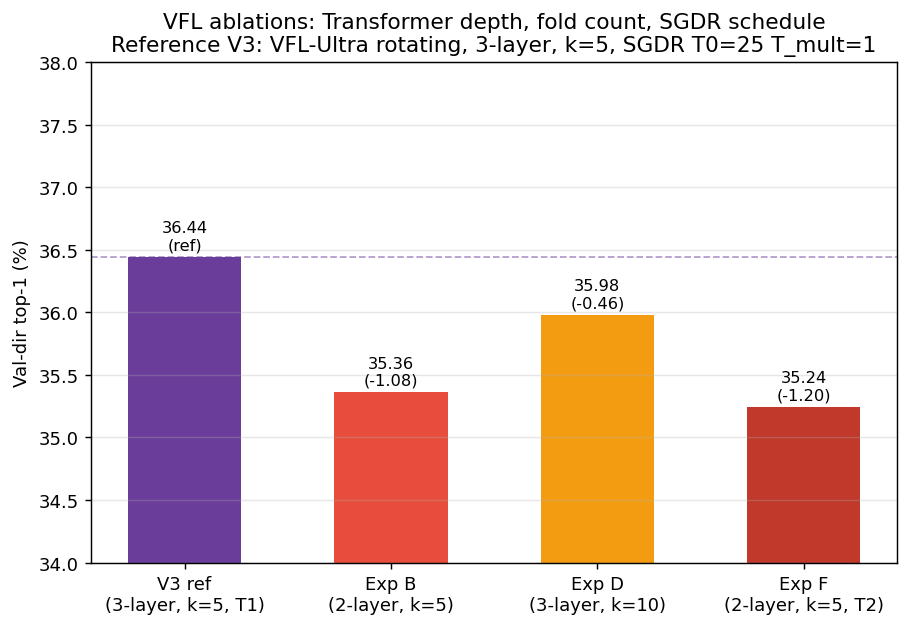
\includegraphics[width=\linewidth]{fig17_ablation_vfl.png}
  \caption{VFL ablations: Transformer depth (2 vs.\ 3 layers,
  $-1.08$\,pp for 2 layers), fold count (5 vs.\ 10, $-0.46$\,pp for 10 folds),
  and SGDR schedule shape ($\leq 0.12$\,pp effect). VFL is data-saturated
  at $k{=}5$ and benefits from a 3rd Transformer block.}
  \label{fig:abla_vfl}
\end{figure}

\begin{figure}[h]
  \centering
  
\includegraphics[width=\linewidth]{fig04_ensemble.png}
  \caption{Track~A ensemble progression. Adding TSM-R50 to the previous 3-model
  R18 ensemble raises 44.03\% to 46.23\%; adding the CE-trained TSM ablation
  reaches \textbf{46.75\%}. The R50 backbone is the dominant component
  ($-1.33$\,pp LOO).}
  \label{fig:ensemble}
\end{figure}

\begin{figure}[h]
  \centering
  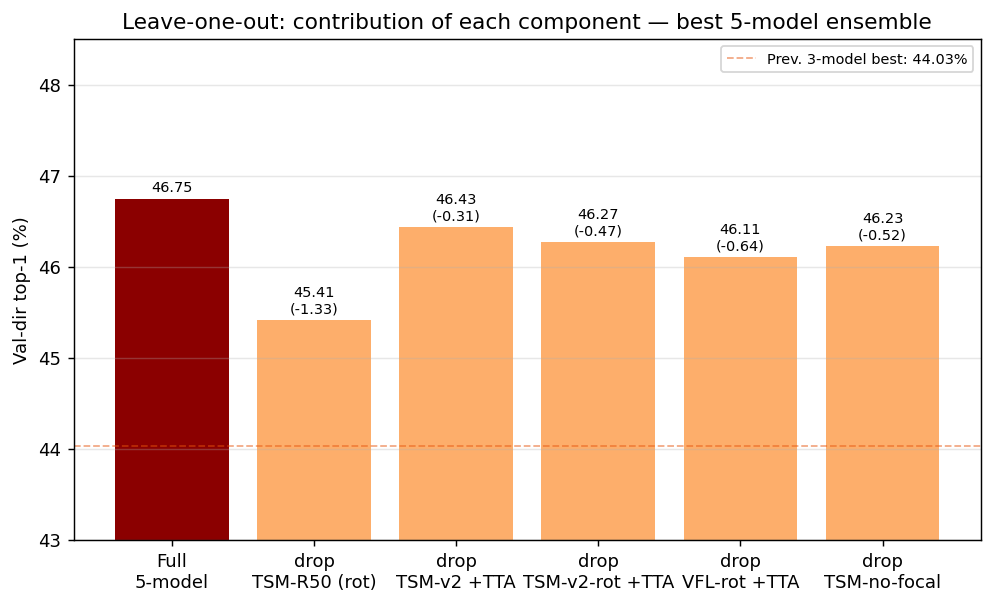
\includegraphics[width=\linewidth]{fig11_leave_one_out.png}
  \caption{Leave-one-out on the 5-model ensemble. The previous 3-model best
  (44.03\%) is the dashed reference. TSM-R50 contributes $-1.33$\,pp alone.}
  \label{fig:loo}
\end{figure}

\begin{figure}[h]
  \centering
  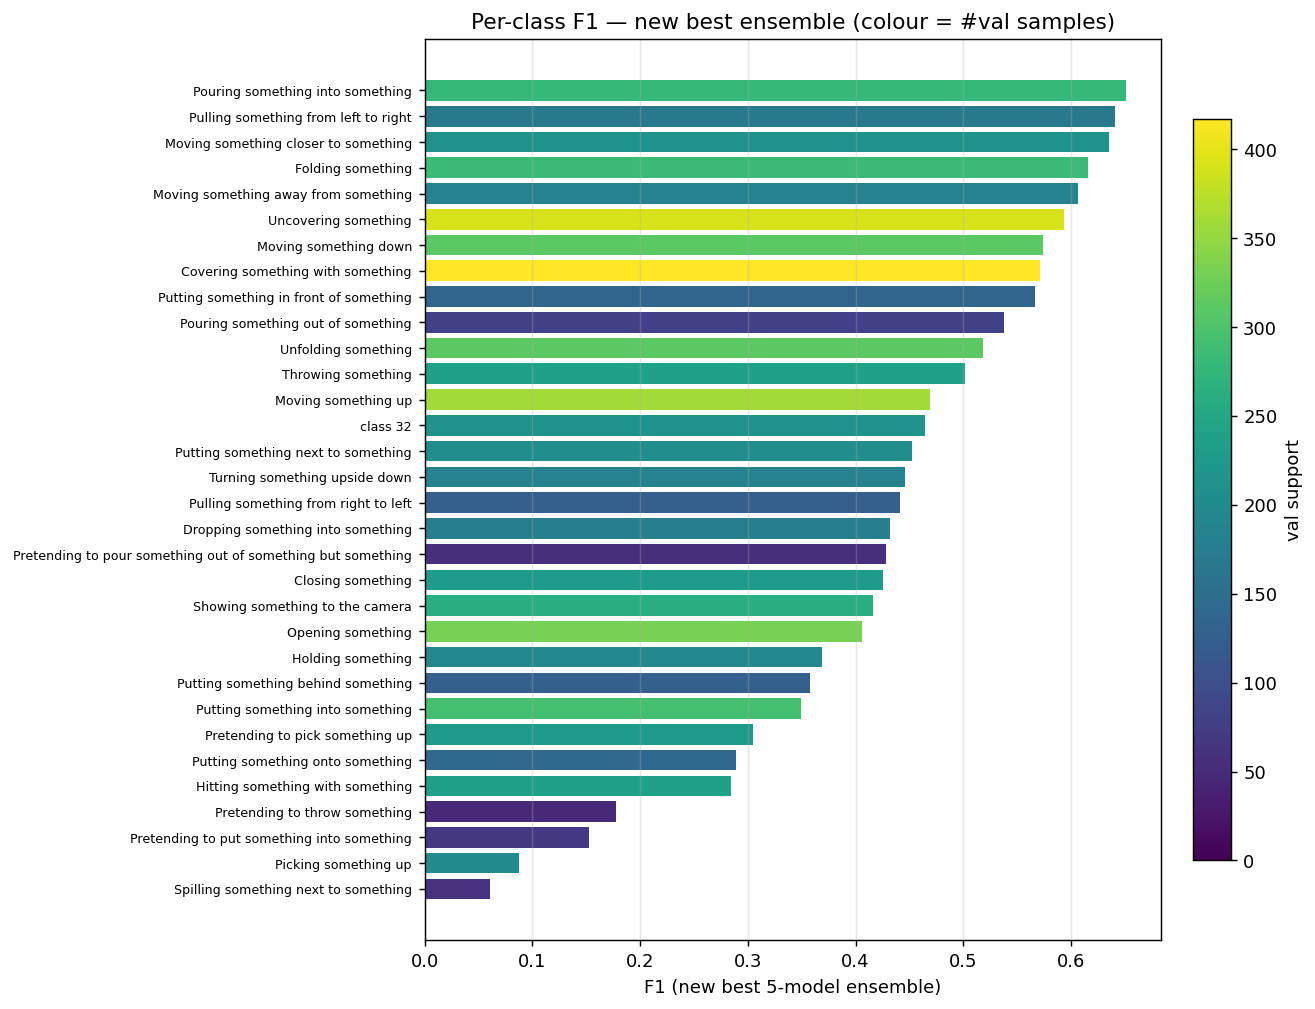
\includegraphics[width=\linewidth]{fig05_per_class_f1.png}
  \caption{Per-class F1 (5-model best ensemble, \texttt{val\_dir}). Directional
  single-object motions score highest; ``pretending'' and direction-ambiguous
  classes score lowest.}
  \label{fig:perclass}
\end{figure}

\begin{figure}[h]
  \centering
  
\includegraphics[width=\linewidth]{fig06_confusion_matrix.png}
  \caption{$33\times33$ confusion matrix (best ensemble, \texttt{val\_dir}).
  Off-diagonal mass concentrates on semantically adjacent pairs (real vs.\
  pretended; fold vs.\ unfold; motion vs.\ \emph{holding}).}
  \label{fig:confmat}
\end{figure}

\begin{figure}[h]
  \centering
  
\includegraphics[width=\linewidth]{fig07_confused_pairs.png}
  \caption{Top-15 confused class pairs. Intent (real vs.\ pretended) and
  temporal direction dominate the error distribution.}
  \label{fig:pairs}
\end{figure}

% =====================================================================
\clearpage
{\small
\bibliographystyle{ieeenat_fullname}
\bibliography{references}
}

\end{document}
